%           ******************************************************
%          **   course         : Memory Technologies             **
%         ***   Presentation   : 04                              ***
%        ****   Topic          : ReTransformer                   ****
%        ****   AUTHOR         : Reza Adinepour                  ****
%         ***   Student ID:    : 402131055                       ***
%          **   Github         : github.com/rezaAdinepour/       **
%           ***************************	***************************

\documentclass[
	12pt, % Set the default font size, options include: 8pt, 9pt, 10pt, 11pt, 12pt, 14pt, 17pt, 20pt
	%t, % Uncomment to vertically align all slide content to the top of the slide, rather than the default centered
	%aspectratio=169, % Uncomment to set the aspect ratio to a 16:9 ratio which matches the aspect ratio of 1080p and 4K screens and projectors
]{beamer}

\graphicspath{{Images/}{./}} % Specifies where to look for included images (trailing slash required)

\usepackage{booktabs} % Allows the use of \toprule, \midrule and \bottomrule for better rules in tables
\usepackage{subcaption}
\usepackage[dvipsnames]{xcolor}

%----------------------------------------------------------------------------------------
%	SELECT LAYOUT THEME
%----------------------------------------------------------------------------------------

% Beamer comes with a number of default layout themes which change the colors and layouts of slides. Below is a list of all themes available, uncomment each in turn to see what they look like.

\usecolortheme{beaver}
\usetheme{Madrid}
\setbeamercolor{section in head/foot}{bg=black}
\setbeamercolor{title}{fg=white, bg=black}
\setbeamercolor{frametitle}{fg=white,bg=black}
\setbeamercolor{block title}{fg=white,bg=black}
\setbeamercolor{item}{fg=black}
\setbeamertemplate{navigation symbols}{}
\setbeamercovered{transparent}

% Add these lines to set the bottom bar to black
\setbeamercolor{author in head/foot}{bg=black, fg=white}
\setbeamercolor{title in head/foot}{bg=gray, fg=white}
\setbeamercolor{date in head/foot}{bg=black, fg=white}
\setbeamercolor{headline}{bg=black}
\setbeamercolor{footline}{bg=black}


%----------------------------------------------------------------------------------------
%	SELECT FONT THEME & FONTS
%----------------------------------------------------------------------------------------

% Beamer comes with several font themes to easily change the fonts used in various parts of the presentation. Review the comments beside each one to decide if you would like to use it. Note that additional options can be specified for several of these font themes, consult the beamer documentation for more information.

\usefonttheme{default} % Typeset using the default sans serif font
%\usefonttheme{serif} % Typeset using the default serif font (make sure a sans font isn't being set as the default font if you use this option!)
%\usefonttheme{structurebold} % Typeset important structure text (titles, headlines, footlines, sidebar, etc) in bold
%\usefonttheme{structureitalicserif} % Typeset important structure text (titles, headlines, footlines, sidebar, etc) in italic serif
%\usefonttheme{structuresmallcapsserif} % Typeset important structure text (titles, headlines, footlines, sidebar, etc) in small caps serif

%------------------------------------------------

%\usepackage{mathptmx} % Use the Times font for serif text
\usepackage{palatino} % Use the Palatino font for serif text

%\usepackage{helvet} % Use the Helvetica font for sans serif text
\usepackage[default]{opensans} % Use the Open Sans font for sans serif text
%\usepackage[default]{FiraSans} % Use the Fira Sans font for sans serif text
%\usepackage[default]{lato} % Use the Lato font for sans serif text

%----------------------------------------------------------------------------------------
%	SELECT INNER THEME
%----------------------------------------------------------------------------------------

% Inner themes change the styling of internal slide elements, for example: bullet points, blocks, bibliography entries, title pages, theorems, etc. Uncomment each theme in turn to see what changes it makes to your presentation.

%\useinnertheme{default}
\useinnertheme{circles}
%\useinnertheme{rectangles}
%\useinnertheme{rounded}
%\useinnertheme{inmargin}

%----------------------------------------------------------------------------------------
%	SELECT OUTER THEME
%----------------------------------------------------------------------------------------

% Outer themes change the overall layout of slides, such as: header and footer lines, sidebars and slide titles. Uncomment each theme in turn to see what changes it makes to your presentation.

%\useoutertheme{default}
%\useoutertheme{infolines}
%\useoutertheme{miniframes}
%\useoutertheme{smoothbars}
%\useoutertheme{sidebar}
%\useoutertheme{split}
%\useoutertheme{shadow}
%\useoutertheme{tree}
%\useoutertheme{smoothtree}

%\setbeamertemplate{footline} % Uncomment this line to remove the footer line in all slides
%\setbeamertemplate{footline}[page number] % Uncomment this line to replace the footer line in all slides with a simple slide count

%\setbeamertemplate{navigation symbols}{} % Uncomment this line to remove the navigation symbols from the bottom of all slides

%----------------------------------------------------------------------------------------
%	PRESENTATION INFORMATION
%----------------------------------------------------------------------------------------

\title[ReTransformer]{ReTransformer} % The short title in the optional parameter appears at the bottom of every slide, the full title in the main parameter is only on the title page

\subtitle{ReRAM-based Processing-in-Memory Architecture for Transformer Acceleration} % Presentation subtitle, remove this command if a subtitle isn't required

\author[Reza Adinepour]{Reza Adinepour} % Presenter name(s), the optional parameter can contain a shortened version to appear on the bottom of every slide, while the main parameter will appear on the title slide

\institute[AUT]{Amirkabir University of Technology (Tehran Polytechnic) \\ \smallskip \href{mailto:adinepour@aut.ac.ir}{\texttt{adinepour@aut.ac.ir}}} % Your institution, the optional parameter can be used for the institution shorthand and will appear on the bottom of every slide after author names, while the required parameter is used on the title slide and can include your email address or additional information on separate lines

\date[\today]{Computer Engineering Department \\ \today} % Presentation date or conference/meeting name, the optional parameter can contain a shortened version to appear on the bottom of every slide, while the required parameter value is output to the title slide

%----------------------------------------------------------------------------------------

\begin{document}

%----------------------------------------------------------------------------------------
%	TITLE SLIDE
%----------------------------------------------------------------------------------------

\begin{frame}\label{start}
	\titlepage % Output the title slide, automatically created using the text entered in the PRESENTATION INFORMATION block above
	\centering
\includegraphics[scale=0.13]{Images/Logo/logo2.png}
\end{frame}

%----------------------------------------------------------------------------------------
%	TABLE OF CONTENTS SLIDE
%----------------------------------------------------------------------------------------

% The table of contents outputs the sections and subsections that appear in your presentation, specified with the standard \section and \subsection commands. You may either display all sections and subsections on one slide with \tableofcontents, or display each section at a time on subsequent slides with \tableofcontents[pausesections]. The latter is useful if you want to step through each section and mention what you will discuss.

\begin{frame}
	\frametitle{Presentation Overview} % Slide title, remove this command for no title
	
	\tableofcontents % Output the table of contents (all sections on one slide)
	%\tableofcontents[pausesections] % Output the table of contents (break sections up across separate slides)
\end{frame}

%----------------------------------------------------------------------------------------
%	PRESENTATION BODY SLIDES
%----------------------------------------------------------------------------------------
\section{Introduction to Transformer Network}
\begin{frame}
	\frametitle{What is a Transformer Network?}
	\begin{columns}
		\begin{column}{0.5\textwidth}
			\begin{enumerate}
				\item 
				Introduced in \textbf{"Attention is All You Need"} (2017)
				
				\item 
				Unlike traditional RNNs and LSTMs, Transformers \textbf{do not} process data sequentially but use a mechanism called \textbf{"self-attention"} to draw global dependencies between input and output.
			\end{enumerate}
		\end{column}
		
		\begin{column}{0.5\textwidth}
			\begin{figure}
				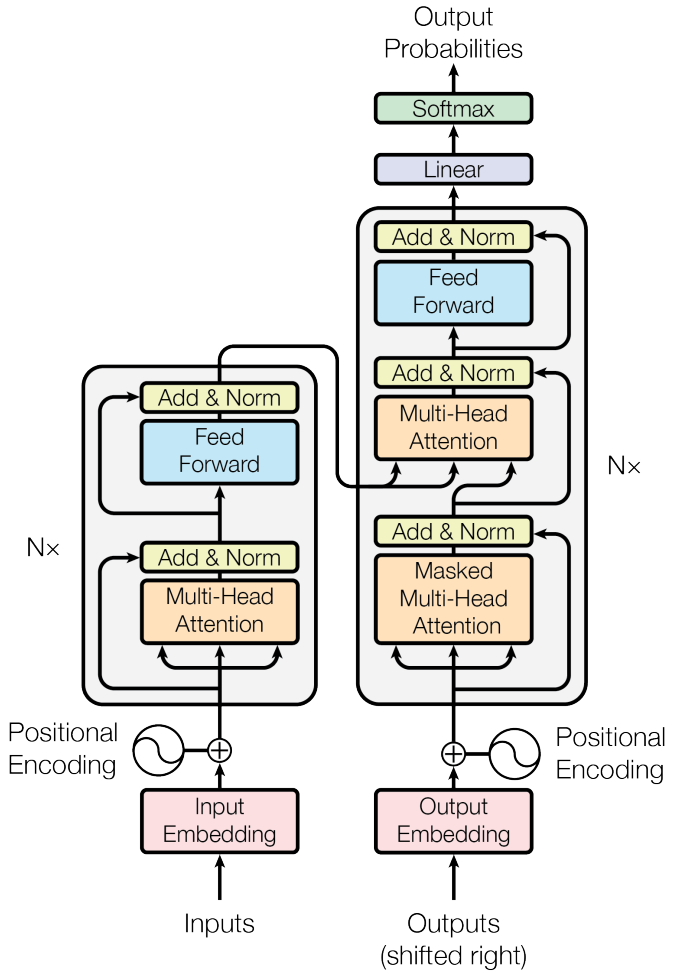
\includegraphics[width=5.3cm]{Images/img1.png}
				\caption{Transformer Architecture}
			\end{figure}
		\end{column}
	\end{columns}			
\end{frame}





\subsection{Why Use Transformers?}
\begin{frame}
	\frametitle{Why Use Transformers?}
	\begin{enumerate}
		\item
		\textbf{Parallelization:}\\ Unlike RNNs, Transformers can process input data in parallel, leading to faster training times.
		
		\item
		\textbf{Self-Attention Mechanism:}\\ This allows the model to weigh the importance of different words in a sentence, capturing long-range dependencies more effectively.
		
		\item 
		\textbf{Scalability:}\\ Transformers can be scaled up effectively, leading to improved performance with more data and larger models.
		
		\item 
		\textbf{Versatility:}\\ They are used in various applications, from machine translation and text generation to image processing and more.
	\end{enumerate}	
\end{frame}





\subsection{Strengths of Transformer}
\begin{frame}
	\frametitle{Strengths of Transformer}
	
	
	\begin{enumerate}
		\item
		\textbf{\textcolor{ForestGreen}{Efficiency:}}\\ Due to parallel processing, they train faster on large datasets.
		
		\item
		\textbf{\textcolor{ForestGreen}{Accuracy:}}\\ State-of-the-art performance in many tasks, particularly in NLP.
		
		\item 
		\textbf{\textcolor{ForestGreen}{Flexibility:}}\\ Applicable to a wide range of tasks beyond language, such as image and speech processing.
		
		\item 
		\textbf{\textcolor{ForestGreen}{Transfer Learning:}}\\ Pre-trained models like BERT and GPT can be fine-tuned for specific tasks with relatively small amounts of data.
	\end{enumerate}
\end{frame}






\subsection{Weaknesses of Transformers}
\begin{frame}
	\frametitle{Weaknesses of Transformers}
	
	\begin{enumerate}
		\item
		\textbf{\textcolor{Red}{Resource-Intensive:}}\\ Require significant computational power and memory, especially for large models.
		
		\item
		\textbf{\textcolor{Red}{Complexity:}}\\ More challenging to understand and implement compared to simpler models.
		
		\item 
		\textbf{\textcolor{Red}{Data Requirements:}}\\ Performance often hinges on the availability of large-scale datasets for pre-training.
		
		\item 
		\textbf{\textcolor{Red}{Inference Speed:}}\\ Performance bottlenecks during inference due to the scaled dot-product attention mechanism.
	\end{enumerate}
\end{frame}







%------------------------------------------------
\section{Motivation}
\begin{frame}
	
	In this paper:
	\frametitle{Motivation}
	
	\begin{enumerate}
		\item
		Developed \textbf{ReTransformer, a ReRAM-based Processing-in-Memory (PIM) architecture} specifically designed to accelerate Transformer models.
		
		\item 
		Implemented \textbf{optimized MatMul operations} to reduce data dependency and intermediate result handling
		
		\item 
		Designed a hybrid softmax mechanism combining in-memory logic and look-up tables for efficient softmax calculations.
		
		\item 
		Introduced a \textbf{sub-matrix pipeline design} for better utilization of ReRAM crossbars and improved throughput.
	\end{enumerate}
\end{frame}

%\begin{frame}
%	\frametitle{Motivation}
%	
%	And Improvements Made is:
%	\begin{enumerate}
%		\item
%		\textbf{Computing Efficiency: }\\
%		ReTransformer improves computing efficiency by 23.21x compared to GPU and 3.25x compared to existing ReRAM-based designs like PipeLayer.
%		
%		\item 
%		\textbf{Power Consumption:}\\
%		Overall power consumption is reduced by 1086x compared to GPU and 2.82x compared to PipeLayer.
%		
%		\item 
%		\textbf{Latency Reduction:}\\
%		Optimized MatMul operations significantly reduce computation latency by 1.32x for smaller models and 1.16x for larger models.
%		
%		\item 
%		\textbf{Softmax Efficiency:}\\
%		The hybrid softmax design lowers power consumption by 32\% compared to traditional CMOS-based designs.
%		
%		\item 
%		\textbf{Throughput Enhancement:}\\
%		The finer granularity sub-matrix pipeline increases computational throughput by 1.18x for both evaluated Transformer models.
%	\end{enumerate}
%\end{frame}



\begin{frame}
	\frametitle{Motivation (Cont.)}
	
	And Improvements Made is:
	\begin{enumerate}
		\item
		\textbf{Computing Efficiency: }\\
		23.21x improvement over GPU, 3.25x over PipeLayer.
		
		\item 
		\textbf{Power Consumption:}\\
		1086x reduction compared to GPU, 2.82x compared to PipeLayer.
		
		\item 
		\textbf{Latency Reduction:}\\
		1.32x for smaller models, 1.16x for larger models.
		
		\item 
		\textbf{Softmax Efficiency:}\\
		32\% lower power consumption compared to traditional CMOS-based designs.
		
		\item 
		\textbf{Throughput Enhancement:}\\
		1.18x increase in computational throughput.
	\end{enumerate}
\end{frame}















\begin{frame}
	\frametitle{Motivation (Cont.)}
	
	This concept use in CNNs and RNNs. but we can't and cant be directly applied to Transformer due to the following reasons:
	
	\begin{enumerate}
		\item 
		\textbf{Matrix-Matrix Multiplication:}\\ 
		Transformers require frequent matrix-matrix multiplications, causing potential slowdowns and reduced efficiency due to intermediate result storage.
		
		\item 
		\textbf{Different Computations:}\\
		Unlike CNNs, Transformers use scaled dot-product attention, necessitating different computational approaches.
		 
		\item 
		\textbf{Finer Pipeline Granularity:}\\
		Transformer accelerators need a more detailed pipeline design compared to the layer-level granularity used in previous designs.
	\end{enumerate}
\end{frame}





%------------------------------------------------
\section{ReRAM Concept}
\begin{frame}
	\frametitle{ReRAM Concept}
	
	\textbf{ReRAM Basics:}
	
	\begin{enumerate}
		\item Is a Non-volatile memory with:
		\begin{itemize}
			\item High density
			\item Low access energy
			\item And support for multi-level cell and 3D integration
		\end{itemize}
		
		\item 
		ReRAM-based Vector-Matrix \& Matrix-Matrix Multiplication:
		\begin{itemize}
			\item Vector-Matrix Multiplication (VMM)
			\item Matrix-Matrix Multiplication (MatMul)
		\end{itemize}
		
		\item
		In-Memory Logic Operations:
		\begin{itemize}
			\item NOR Logic
			\item XOR Logic
			\item And other Logic Operations
		\end{itemize}
	\end{enumerate}	
\end{frame}



\subsection{Vector-Matrix Multiplication (VMM)}
\begin{frame}
	\frametitle{Vector-Matrix Multiplication (VMM)}
	\begin{columns}
		\begin{column}{0.5\textwidth}
			\begin{enumerate}
				\item 
				Conductance of ReRAM cells represents elements in a matrix.
				
				\item 
				Input voltage vector $(V_I=[v_0, v_1, v_2, v_3])$ fed to word lines (WLs) generates output current through bit lines (BLs).
				
				\item 
				One read cycle completes the VMM operation.
			\end{enumerate}
		\end{column}
		
		\begin{column}{0.5\textwidth}
			\begin{figure}
				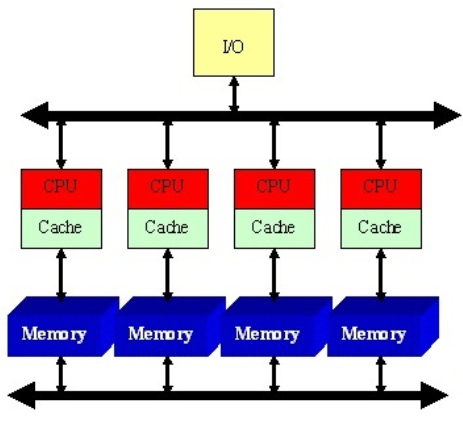
\includegraphics[width=6.4cm]{Images/img2.png}
				\caption{ReRAM-based vector-matrix multiplication}
			\end{figure}
		\end{column}
	\end{columns}
	According to Kirchhoff’s law the output current calculate as bellow: \\
	$$ i_j=\sum_{i=0}^{3} \frac{v_i}{R(i,j)}=\sum_{i=0}^{3}v_iG(i, j) $$		
\end{frame}



\subsection{Matrix-Matrix Multiplication (MatMul)}
\begin{frame}
	\frametitle{Matrix-Matrix Multiplication (MatMul)}
	\begin{enumerate}
		\item Input matrix separated into vectors for sequential VMM operations
		\item Results of VMM operations combined to obtain MatMul results
	\end{enumerate}
\end{frame}



\subsection{In-Memory Logic Operations}
\begin{frame}
	\frametitle{In-Memory Logic Operations}
	\begin{columns}
		\begin{column}{0.5\textwidth}
			\begin{enumerate}
				\item 
				\textbf{NOR Logic:}\\ Uses high and low conductance values to represent logic states. Operations performed using specific voltage settings.
				
				\item 
				\textbf{XOR Logic:}\\ Implemented using a combination of OR and NAND operations, leveraging ReRAM's programmable conductance.
				
				\item 
				\textbf{Other Logic Operations:}\\ INV and OR implemented in one or two cycles respectively.
			\end{enumerate}
		\end{column}
		
		\begin{column}{0.5\textwidth}
			\begin{figure}
				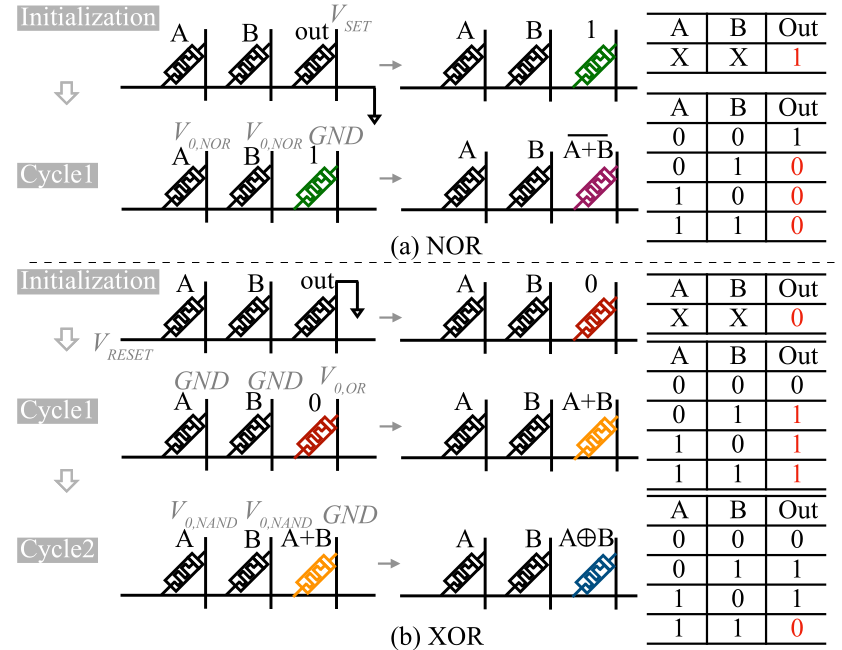
\includegraphics[width=6.3cm]{Images/img3.png}
				\caption{ReRAM-based in-memory logic: (a) NOR, (b) XOR.}
			\end{figure}
		\end{column}
	\end{columns}		
\end{frame}
%------------------------------------------------





\section{Overall Architecture}
\begin{frame}
	\frametitle{Overall Architecture}
	A ReRAM-based PIM module is divided into three types of functional components:
	\begin{columns}
		\begin{column}{0.5\textwidth}
			\begin{enumerate}
				\item 
				\textbf{Processing Subarrays:}\\
				Execute computations such as MatMul and feed-forward operations.
				
				\item 
				\textbf{Buffer Subarrays:}\\ 
				Serve as caches to store intermediate data and results.
				
				\item 
				\textbf{Memory Subarrays:}\\
				Store original input data and final output results.
			\end{enumerate}
		\end{column}
		
		\begin{column}{0.5\textwidth}
			\begin{figure}
				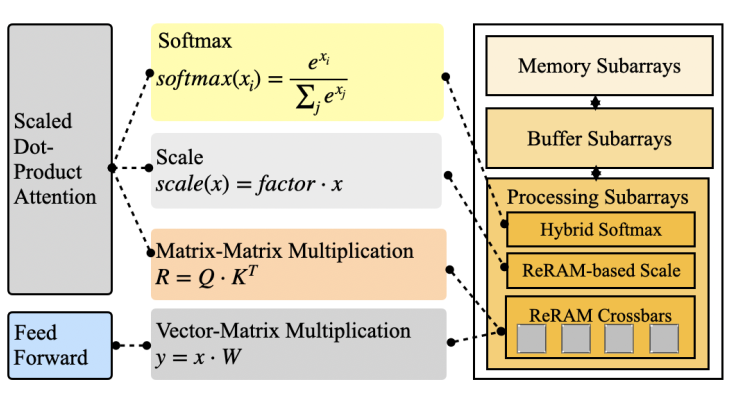
\includegraphics[width=6.3cm]{Images/img4.png}
				\caption{Overview of the proposed ReRAM-based PIM design for Transformer}
			\end{figure}
		\end{column}
	\end{columns}		
\end{frame}




\subsection{Key Features}
\begin{frame}
	\frametitle{Key Features}
	\begin{columns}
		\begin{column}{0.5\textwidth}
			\begin{enumerate}
				\item 
				\textbf{ReRAM Crossbars:}\\
				Enable efficient in-memory computations.
%				Enable efficient in-memory computations, reducing data movement and improving speed.
				
				\item 
				\textbf{Optimized MatMul:}\\ 
				Reduces data dependency and intermediate writes.
%				Decomposes matrix multiplication into stages to avoid frequent intermediate writes, enhancing speed and efficiency.
				
				\item 
				\textbf{Hybrid Softmax Mechanism:}\\
				Combines in-memory logic with look-up tables for efficiency.
%				Combines in-memory logic with look-up tables for efficient softmax calculations, reducing power consumption.

				\item 
				\textbf{Sub-Matrix Pipeline:}\\
				Slices input matrices for parallel processing.
%				Slices input matrices into smaller segments to maximize resource utilization and improve throughput.
			\end{enumerate}
		\end{column}
		
		\begin{column}{0.5\textwidth}
			\begin{figure}
				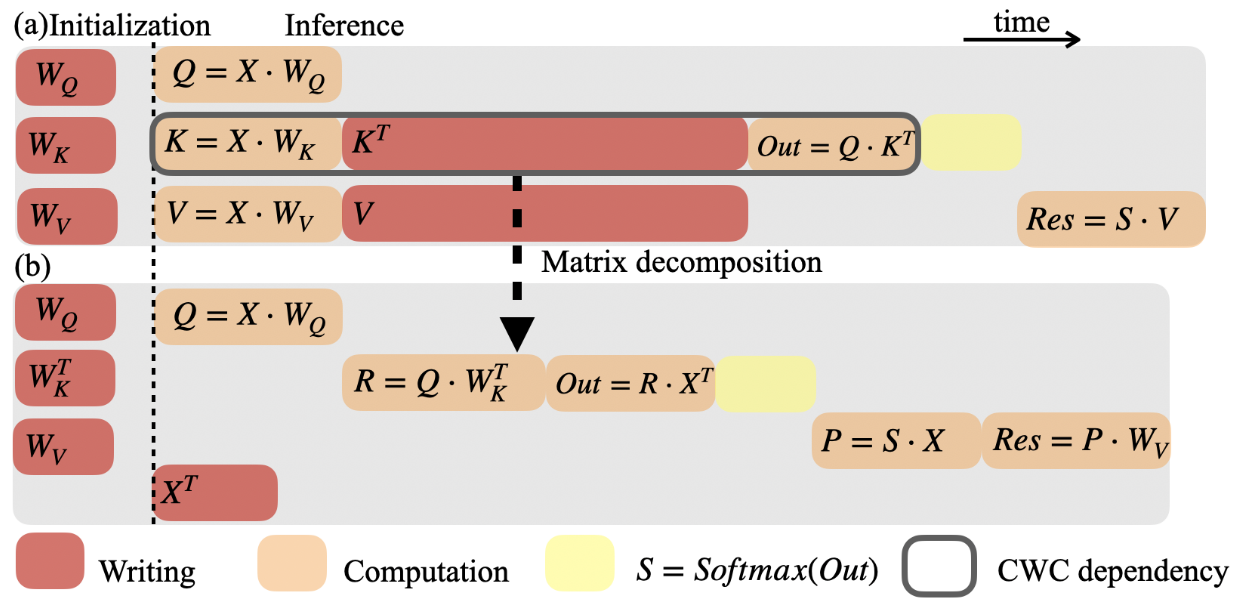
\includegraphics[width=6.3cm]{Images/img5.png}
				\caption{Remove data dependency in scaled dot-product
					attention layer: (a) a CWC dependency caused by the in-
					termediate result K. (b) The optimized MatMul eliminates
					the CWC dependency by decomposing the computation into
					two cascaded multiplications.}
			\end{figure}
		\end{column}
	\end{columns}		
\end{frame}




\subsection{Workflow}
\begin{frame}
	\frametitle{Workflow}
	
	\begin{enumerate}
		\item 
		\textbf{Data Loading:}\\
		Input data is stored in memory subarrays.
		
		\item 
		\textbf{Computation:}\\
		Processing subarrays perform operations using data from buffer subarrays.
		
		\item 
		\textbf{Intermediate Handling:}\\
		Buffer subarrays temporarily store intermediate results, reducing the need for frequent memory writes.
		
		\item 
		\textbf{Output Storage:}\\
		Final results are stored back in memory subarrays.
	\end{enumerate}	
\end{frame}
%--------------------------------------------------








\section{Experimental Setup}
\begin{frame}
	\frametitle{Experimental Setup}
	
	\begin{enumerate}
		\item 
		\textbf{Configurations:}\\
		\begin{itemize}
			\item GPU: NVIDIA TITAN RTX, 24GB memory, 672 GB/s bandwidth.
			\item ReTransformer: ReRAM crossbar arrays, 2-bit cell precision, 128x128 subarray size.
		\end{itemize}
		
		\item 
		\textbf{Evaluation Metrics:}\\
		\begin{itemize}
			\item Computing Efficiency: Operations per second per watt.
			\item Power Consumption: Total power used during computations.
		\end{itemize}
	\end{enumerate}	
\end{frame}
%--------------------------------------------------











\section{Results and Analysis}
\begin{frame}
	\frametitle{Results and Analysis}
	\textbf{MatMul Optimization:}\\
	Reduces computation latency by 1.32x for Model A and 1.16x for Model B.
	
	\begin{figure}
		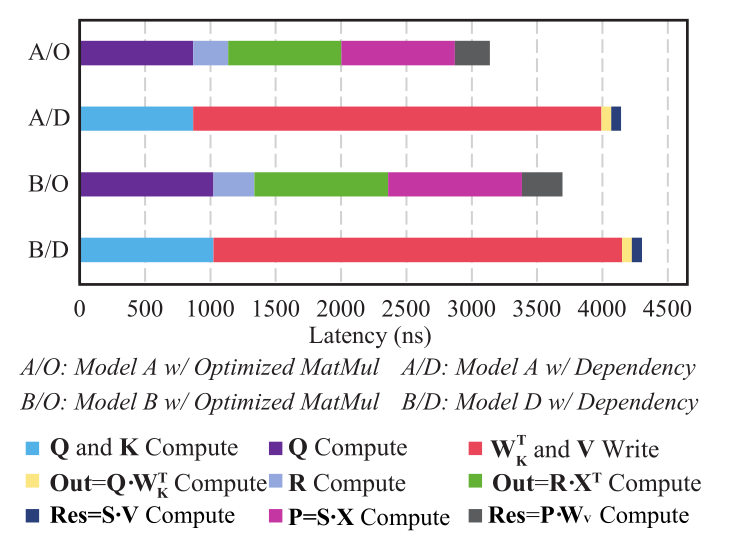
\includegraphics[width=7.5cm]{Images/img6.png}
		\caption{MatMul computation latency comparisons}
	\end{figure}
\end{frame}



\begin{frame}
	\frametitle{Results and Analysis (Cont.)}
	\textbf{Hybrid Softmax Efficiency:}\\
	Lowers power consumption by 32\% compared to CMOS-based design.
	
	\begin{figure}
		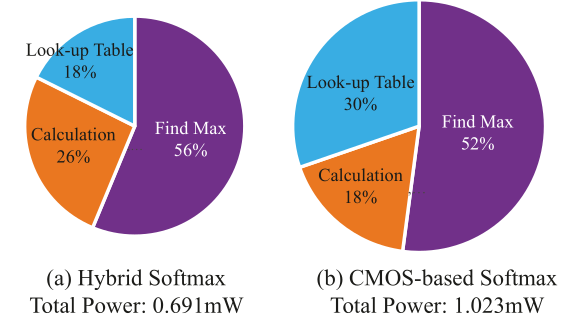
\includegraphics[width=7.5cm]{Images/img7.png}
		\caption{Softmax design comparison}
	\end{figure}
\end{frame}



\begin{frame}
	\frametitle{Results and Analysis (Cont.)}
	\textbf{Pipeline Performance:}\\
	Finer granularity pipeline improves throughput by 1.18x for both models.
	
	\begin{table}[h]
		\centering
		\begin{tabular}{c|c|c|c}
			\hline
			\textbf{Model} & \textbf{Layer} & \textbf{Finer} & \textbf{Improvement} \\
			\hline
			\textbf{Model A} & 69.24 GOPs/s & 81.85 GOPs/s & 1.18x \\ \hline
			\textbf{Model B}& 67.89 GOPs/s & 80.07 GOPs/s & 1.18x \\
			\hline
		\end{tabular}
		\caption{Performance comparison of two pipeline designs}
	\end{table}
\end{frame}



\begin{frame}
	\frametitle{Results and Analysis (Cont.)}
	\textbf{Overall Comparison:}\\
	
	\begin{enumerate}
		\item ReTransformer achieves 23.21x improvement in computing efficiency and 1086x reduction in power consumption compared to GPU.
		
		\item Compared to PipeLayer, ReTransformer improves computing efficiency by 3.25x and reduces power by 2.82x.
		
		
	\end{enumerate}
	
	\begin{figure}
		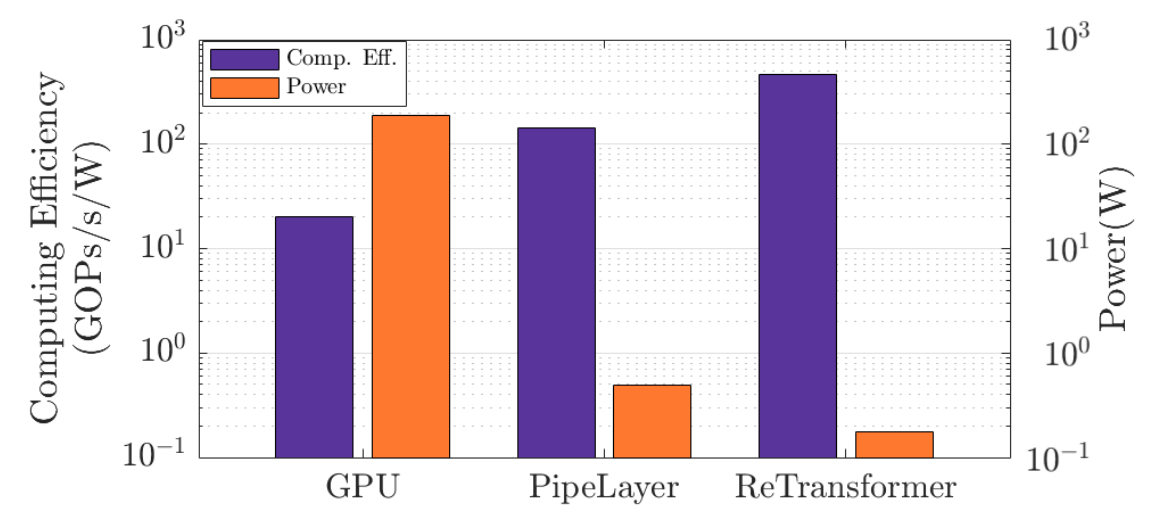
\includegraphics[width=8.5cm]{Images/img8.png}
		\caption{Performance comparison with GPU and PipeLayer}
	\end{figure}
\end{frame}







\section{References}
\begin{frame}{References}
	
	\hyperlink{start}{\beamerreturnbutton{Back to start}}
	
	\nocite{bibitem1}
	\nocite{*}
	\bibliographystyle{IEEEtran} 
	\bibliography{ref}
	
\end{frame}


%----------------------------------------------------------------------------------------
%	CLOSING SLIDE
%----------------------------------------------------------------------------------------

\begin{frame}[plain] % The optional argument 'plain' hides the headline and footline
	\begin{center}
		{\Huge The End}
		
		\bigskip\bigskip % Vertical whitespace
		
		{\LARGE Questions? Comments?}\\
		You can find this slides here:\\
		\textcolor{blue}{\href{https://github.com/M-Sc-AUT/M.Sc-Computer-Architecture/tree/main/Memory Technologies}{\texttt{github.com/M-Sc-AUT/M.Sc-Computer-Architecture/Memory Technologies}}}
		
		I delivered three presentations this semester on the following topics:
		\begin{enumerate}
			\item Multiprocessors shared-memory Architecture
			\item Exploring CACTI and NVSIM Simulators
			\item Exploring DRAMSim and SimpleScaler Simulators
		\end{enumerate}
	\end{center}
\end{frame}

%----------------------------------------------------------------------------------------

\end{document} 